\section{Membuat APlikasi Monitoring Berbasis Android}
\subsection{Android}
 \begin{figure}[H]
    \centering
    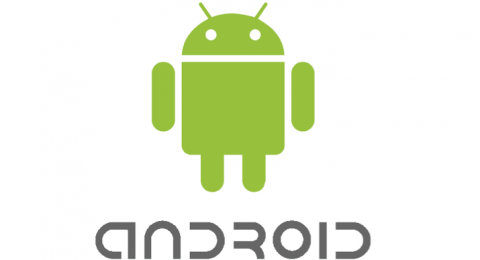
\includegraphics[width=0.9\textwidth]{figures/android.png}
    \caption{Logo Android}
    \label{print}
    \end{figure}
    
    
    \par Android adalah sistem operasi yang dirancang oleh Google dengan basis kernel Linux untuk mendukung kinerja perangkat elektronik layar sentuh, seperti tablet atau smartphone. Jadi, android digunakan dengan sentuhan, gesekan ataupun ketukan pada layar gadget anda.\\
    \par Android  salah satu sistem operasi atau \textit{operating system} berbasis \textit{mobile} yang sangat banyak di gunakan sekarang ini. Utamanya pada telepon pintar \textit{(smartphone)} ataupun tablet.\\
    \par Android bersifat \textit{open source} atau bebas digunakan, dimodifikasi, diperbaiki dan didistribusikan oleh para pembuat ataupun pengembang perangkat lunak. Dengan sifat \textit{open source} perusahaan teknologi bebas menggunakan OS ini diperangkatnya tanpa lisensi alias gratis.
    \par Kelebihan Android yaitu sebagai berikut :
    \begin{enumerate}
        \item Merupakan Sistem Operasi Open Source
\par Siapa saja bisa menggunakannya secara gratis. Para \textit{developer} atau pengembang dimudahkan untuk mengoptimalkan dan mengembangkan OS ini untuk \textit{smartphone} yang dibuatnya.

\item Memiliki Banyak Dukungan Aplikasi
\par Hal ini juga tidak lepas dari sifat Android yang merupakan sistem operasi \textit{Open Source}. Pengembang pun diizinkan untuk mengembangkan aplikasi berbasis source code dari Android.

\par Oleh karena itu, jika Anda masuk ke \textit{Play Store}, akan ditemukan banyak sekali ribuan aplikasi yang sesuai dengan kebutuhan pengguna.

\item Mudah dimodifikasi
\par Banyak komponen yang bisa Anda atur ulang atau dimodifikasi, mulai dari ROM  hinga custom \textit{overclock} pada sistem operasi. Hal ini bisa berpengaruh terhadap performa ponsel pintar berbasis Android agar bisa bekerja lebih cepat dan sesuai dengan keinginan.
\end{enumerate}
\par Kekurangan Android yaitu sebagai berikut :
\begin{enumerate}
    \item  Kerja sistemnya cukup berat
    \par Hal ini menyebabkan banyak memori yang dibutuhkan, baik RAM maupun ROM. Bagi \textit{smartphone} yang memiliki RAM dan ROM berkapasitas kecil, tentunya akan menghambat performanya.
    \item Hasil modifikasi sering menyebabkan sistem bekerja tidak stabil dan kurang optimal
    \par Adakalanya hasil modifikasi mengakibatkan OS menjadi sedikit lelet dan kurang responsif. Nantinya, bisa berpengaruh pada hardware sehingga menjadi cepat panas dan kapasitas memori lebih mudah bocor.
    \item Kurang responsif jika disandingkan dengan spesifikasi hardware yang tidak baik
    \par Hal tersebut berkaitan dengan kapasitas RAM, ROM, dan kecepatan prosesor yang digunakan pada \textit{smartphone.}
\end{enumerate}
\subsection{Perkembangan Android}
    \begin{figure}[H]
    \centering
    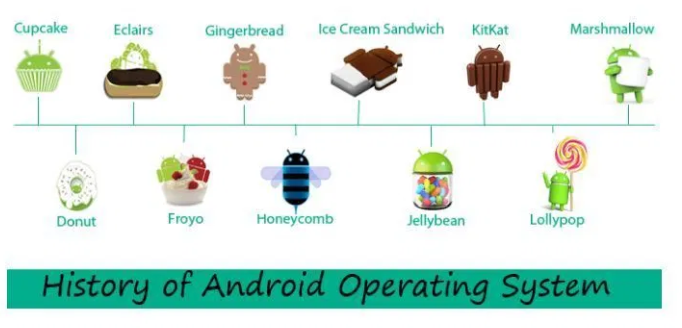
\includegraphics[width=0.9\textwidth]{figures/android2.png}
    \caption{Perkembangan Android}
    \label{print}
    \end{figure}

\par Sejak tahun 2009, Android mulai dikembangakn dengan kode yang dinamai berdasarkan makanan pencuci mulut. Tiap versi dirilis sesuai dengan urutan abjad.
\begin{enumerate}
    \item Astro 1.0
    \par Versi ini pertama kali dirilis pada 23 September 2008 yang awalnya akan dinamai dengan nama “Astro” saja. Namun karena alasan hak cipta dan trademark, nama ini tidak jadi disematkan pada versi pertama ini. Versi Astro 1.0 pertama kali digunakan oleh smartphone HTC Dream.
    \item Bender 1.1
    \par Bender 1.1 dirilis pada 9 Februari 2009. Lagi-lagi, versi dari OS ini mengalami masalah penamaan yang serupa dengan versi sebelumnya. Awalnya, versi ini diberi nama Bender dan dirilis untuk perangkat T-Mobile G1 saja.
    \item Cupcake 1.5
    \par Cupcake 1.5 dirilis pada 30 April 2009. Dimulai dari versi ini, penamaan menggunakan nama makanan pencuci mulut. Karena merupakan versi ketiga, makan penamaannya dimulai dengan huruf “C” dan “Cupcake” menjadi nama resminya.
    \item Donut 1.6
    \par Versi yang dirilis pada 15 September 2009 ini memiliki peningkatan pada fitur pencarian dan UI yang lebih user friendly. Donut 1.6 sudah mendukung teknologi CDMA/EVDO, 802.1 x, VPNs.
    \item Eclair 2.0 – 2.1
    \par Eclair 2.0 – 2.1 dirilis pada 3 Desember 2009 dan untuk pertama kalinya membawa fitur baru, yaitu Google Maps yang dapat membantu pengguna dalam bepergian.
    \item Froyo 2.2
    \par Froyo atau disingkat dari frozen yoghurt merupakan versi Android yang rilis pada 20 Mei 2010.

\par Perubahan umumnya antara lain adalah adanya dukungan Adobe Flash 10.1, kecepatan kinerja, intergrasi V8 JavaScript engine, pemasangan aplikasi dalam SD Card, kemampuan Wi-Fi Hotspot portable, dan kemampuan auto update dalam aplikasi Android Market.

\item Gingerbread 2.3
\par Versi ini dirilis pada 6 Desember 2010 dan terdapat perubahan dalam peningkatan kemampuan gaming, peningkatan fungsi copy paste, User Interface, dukungan format video VP8 dan WebM, hingga dukungan jumlah kamera lebih dari satu.
\item Honeycomb 3.0/3.1
\par Versi yang diluncurkan pada 22 Februari 2011 ini merupakan OS yang didesain khusus untuk pengoptimalan penggunaan pada tablet PC. Versi Honeycomb ini juga mendukung multi prosesor dan akselerasi hardware untuk grafis.

\item Ice Cream Sandwich 4.0
\par Ice Cream Sandwich 4.0 diluncurkan tanggal 19 Oktober 2011 dan membawa fitur Honeycomb untuk smartphone dengan membawa fitur brau, seperti membuka kunci dengan pengenala wajah, perangkat tambahan fotografi, hingga berbagi informasi menggunakan NFC.
\item Jelly Bean 4,1/4.2/4.3
\par Di tahun 2012, android mengeluarkan versi Jelly Bean. Lewat versi Jelly Bean (4.1) Google mulai menerapkan teknologi asisten digital Google Now yang bisa diakses langsung dari homescreen.

\par Pada versi 4.2 terdapat fitur photo sphere untuk panorama, daydream sebagai screensaver, power control, dsb. Sedangkan versi 4.3 merupakan pembaharuan dari versi sebelumnya.
\item KitKat 4.4
\par KitKat 4.4 diluncurkan pada 3 September 2013. Versi yang sebelumnya bernama Key Lime Pie ini membawa peningkatan yang cukup signifikan karena Google lebih fokus meningkatkan user experience.

\par Versi ini dioptimalkan untuk berjalan pada rentang yang lebih besar dari versi Android sebelumnya. Disarankan perangkat harus memiliki minimal RAM 512 MB.

\item Lollipop 5.0
\par Versi yang diluncurkan pada 12 November 2014 ini tersedia secara resmi melalui over the air (OTA). Perubahan yang paling menonjol dalam versi ini adalah User Interface yang didesain ulang dan dibangun dengan “material design”.
\item Marshmallow 6.0
\par Sistem operasi ini membawa banyak fitur canggih, mulai dari Doze untuk menghemat baterai, dukungan USB tipe C, percobaan multi window, sensor sidik jari untuk buka kunci layar, hingga pengguna bisa memakai dua aplikasi berbeda dalam satu layar.
\item Nougat 7.0
\par Versi ini merupakan salah satu upgrade terbesar dalam sistem operasi Android. Nougat 7.0 merupakan pengembangan dari Marshmallow yang meningkatkan performa dan interface yang lebih intuitif.
\item Oreo 8.0
\par Orea 8.0 dirilis pada 2017 dengan menambah lebih banyak fitur multi tasking dan perombakan bagian notifikasi. Pengguna bisa mengatur mana saja notifikasi yang ingin ditampilkan.

\par Tampilan UI-nya juga lebih rapi dan segar, serta difokuskan untuk memudahkan pengguna mengakses aplikasi dan mencari informasi.
\item Pie 9.0
\par Versi yang diluncurkan pada Agustus 2018 ini mengganti tiga tombol navigasi dengan tombol tunggal berbentuk elips. Android Pie disokong dengan kemampuan kecerdasan buatan (AI) yang menjadikannya bisa mempelajari pola penggunaan secara otomatis.
\end{enumerate}